\textbf{Ejemplo 1}\\

Una persona está pensando en construir un parqueadero, para tal fin, toma en alquiler un lote por un plazo de 5 años. El costo de la construcción, incluidos los impuestos y las licencias, es de 15.000.000 COP; se estima que los ingresos después de descontar el valor de los arriendos e impuestos, es decir, los ingresos netos, serán 5.000.000 COP, los cuales crecerán cada año aproximadamente de acuerdo al índice de inflación que se estima en un 20\% período anual vencido. Si el inversionista gana normalmente en todos sus negocios un 35\% período anual vencido. ¿Es aconsejable este negocio?
\\

\textbf{Solución.}\\
\begin{center}
    \renewcommand{\arraystretch}{1.5} %Margenes de las celdas
    \begin{longtable}{|c|c|c|} %Creacion de una cuadricula de 4 columnas
        \hline % Crea una linea horizonal arriba
        \rowcolor[HTML]{FFB183} %Define el color de la primera fila
        %%% INICIO ASIGNACION PERIODO FOCAL %%%%
        %%%INICIO TITULO
        %MEZCLAR 3 COLUMNAS EN UNA SOLA
        \multicolumn{3}{|c|}{\cellcolor[HTML]{FFB183}\textbf{1. Asignación periodo focal}}                                                                                                                                            \\ \hline
        %%FIN TITULO
        \multicolumn{3}{|c|}{$pf : 0 pav$}                                                                                                                                                                                            \\
        %%%FIN ASIGNACION PERIODO FOCAL
        \hline
        %%%% INICIO DECLARACION DE VARIABLES
        %%%INICIO TITULO
        \multicolumn{3}{|c|}{\cellcolor[HTML]{FFB183}\textbf{2. Declaración de variables}}                                                                                                                                            \\ \hline
        \multicolumn{1}{|c|}{\cellcolor[HTML]{FFB183}\textbf{Valores monetarios}}    & \multicolumn{1}{c|}{\cellcolor[HTML]{FFB183}\textbf{Valores no monetarios}} & \multicolumn{1}{c|}{\cellcolor[HTML]{FFB183}\textbf{Incógnitas}} \\ \hline
        %%%FIN TITULO
        %Cada & hace referencia al paso de la siguiente columna
        %Cada \\ hace referencia a un salto de linea
        $\textbf{Inversión inicial} = $ $15\text{.}000\text{.}000 \text{ COP}$       & $i_{1} = 20\% pav$                                                          &                                                                  \\
        $\textbf{Ingresos netos primer año} =$ $5\text{.}000\text{.}000 \text{ COP}$ & $i_{2} = TIO = 35\% pav$                                                    & $i = TIR = ?\% pav$                                              \\
                                                                                     & $n = 5 pav$                                                                 &                                                                  \\

        \hline
        %%% FIN DECLARACION DE VARIABLES
        %%%INICIO DIAGRAMA DE FLUJO
        %%INICIO TITULO
        \multicolumn{3}{|c|}{\cellcolor[HTML]{FFB183}\textbf{3. Diagrama de flujo de caja}}                                                                                                                                           \\ \hline
        %%FIN TITULO
        %%%%%%%%%%%%% INSERCIÓN DE LA IMAGEN
        %Mezclamos 3 columnas y pondremos el dibujo
        %Deberán descargar las imágenes respectivas del drive y pegarlas en la carpeta
        %n_capitulo/img/ejemplos/1/capitulo1ejemplo1.pdf  (el /1/ es el numero del ejemplo)
        \multicolumn{3}{|c|}{ 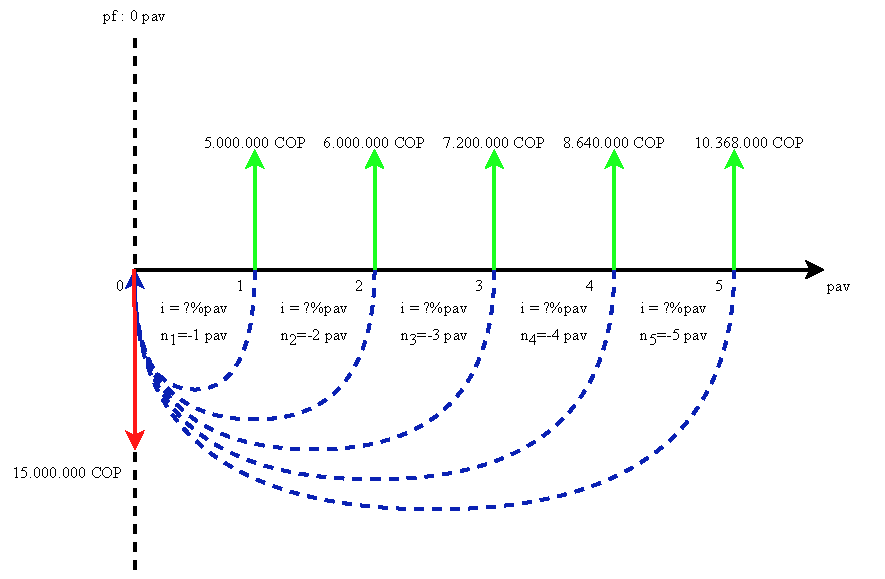
\includegraphics[scale=0.9]{ejemplos/1/Graf1Ej1Cap11.pdf} }
        \\ \hline
        %%%%%%%%%%%%% FIN INSERCIÓN DE IMAGEN
        %%%FIN DIAGRAMA DE FLUJO
        %%%INICIO DECLARACION DE FORMULAS
        %%INICIO TITULO
        \multicolumn{3}{|c|}{\cellcolor[HTML]{FFB183}\textbf{4. Declaración de fórmulas}}                                                                                                                                             \\ \hline
        %%FIN TITULO
        %%%%%%%%%%% INICIO MATEMÁTICAS
        \multicolumn{3}{|c|}{$F = P(1+i)^n \hspace{0.3cm} $ Valor futuro.}                                                                                                                                                     \\
        \multicolumn{3}{|c|}{$VPN =\sum F_{n}(1+i)^{-n} $ Valor presente neto.}                                                                                                                                                       \\ \hline
        %%%%%%%%%% FIN MATEMÁTICAS
        %%%FIN DECLARACION DE FORMULAS
        %%%INICIO DESARROLLO MATEMATICO
        %%INICIO TITULO
        \multicolumn{3}{|c|}{\cellcolor[HTML]{FFB183}\textbf{5. Desarrollo matemático}}                                                                                                                                               \\ \hline
        %%FIN TITULO
        %%%%%%%%%%% INICIO MATEMÁTICAS
        \multicolumn{3}{|c|}{$F_1 = $ $5\text{.}000\text{.}000 \text{ COP}$  $(1 + 0.2)^{1} = $ $6\text{.}000\text{.}000 \text{ COP}$ }                                                                                               \\
        \multicolumn{3}{|c|}{$F_2 = $ $6\text{.}000\text{.}000 \text{ COP}$  $(1 + 0.2)^{1} = $ $7\text{.}200\text{.}000 \text{ COP}$ }                                                                                               \\
        \multicolumn{3}{|c|}{$F_3 = $ $7\text{.}200\text{.}000 \text{ COP}$  $(1 + 0.2)^{1} = $ $8\text{.}640\text{.}000 \text{ COP}$ }                                                                                               \\
        \multicolumn{3}{|c|}{$F_4 = $ $8\text{.}640\text{.}000 \text{ COP}$  $(1 + 0.2)^{1} = $ $10\text{.}368\text{.}000 \text{ COP}$ }                                                                                              \\
        \multicolumn{3}{|c|}{ $ VPN = -15\text{ COP} + 5\text{ COP}(1+i)^{-1} + 6\text{ COP}(1+i)^{-2} + 7.2\text{ COP}(1+i)^{-3} +$  }                                                                                               \\
        \multicolumn{3}{|c|}{$ 8,64\text{ COP}(1+i)^{-4} + 10,368\text{ COP}(1+i)^{-5}$}                                                                                                                                              \\
        \multicolumn{3}{|c|}{$\textbf{La TIR la tasa en la cual el VPN se hace cero:}  $}                                                                                                                                             \\

        \multicolumn{3}{|c|}{$ VPN = -15\text{ COP} + 5\text{ COP}(1+i)^{-1} + 6\text{ COP}(1+i)^{-2} + 7.2\text{ COP}(1+i)^{-3}$}                                                                                                    \\
        \multicolumn{3}{|c|}{$8,64\text{ COP}(1+i)^{-4} + 10,368\text{ COP}(1+i)^{-5} = 0$}                                                                                                                                           \\

        \multicolumn{3}{|c|}{$\textbf{La solucion manual requiere usar la interpolación, para ello escogemos valores para i no }  $}                                                                                                  \\
        \multicolumn{3}{|c|}{$ \textbf{muy alejados entre sí de tal forma que la función sea una vez positiva y otra negativa, así:}$}                                                                                                \\
        \multicolumn{3}{|c|}{$ \textit{Primer ensayo: }$}                                                                                                                                                                             \\
        \multicolumn{3}{|c|}{$ \textit{i = 34\% pav}$}                                                                                                                                                                                \\
        \multicolumn{3}{|c|}{$ VPN = -15\text{ COP} + 5\text{ COP}(1+0.34)^{-1} + 6\text{ COP}(1+0.34)^{-2} + 7.2\text{ COP}(1+0.34)^{-3}$}                                                                                           \\
        \multicolumn{3}{|c|}{$+8,64COP(1+0.34)^{-4} + 10,368\text{ COP}(1+0.34)^{-5}=0.144763$}                                                                                                                                       \\
        \multicolumn{3}{|c|}{$ \textit{Segundo ensayo: }$}                                                                                                                                                                            \\
        \multicolumn{3}{|c|}{$ \textit{i = 35\% pav}$}                                                                                                                                                                                \\
        \multicolumn{3}{|c|}{$ VPN = -15\text{ COP} + 5\text{ COP}(1+0.35)^{-1} + 6\text{ COP}(1+0.35)^{-2} + 7.2\text{ COP}(1+0.35)^{-3} +$}                                                                                         \\
        \multicolumn{3}{|c|}{$8,64\text{ COP}(1+0.35)^{-4} + 10,368\text{ COP}(1+0.35)^{-5} = -0.164298$}                                                                                                                             \\
        \multicolumn{3}{|c|}{$ \textit{Se toman los resultados correspondientes al 34\%  y a 35\% por ser los más}$}                                                                                                                  \\
        \multicolumn{3}{|c|}{$  \textit{cercanos y los que presentan diferente signo y los colocaremos de la siguiente forma:}$}                                                                                                      \\
        \multicolumn{3}{|c|}{$ \textit{Se plantea la siguiente proporción:} $}                                                                                                                                                        \\
        \multicolumn{3}{|c|}{$ \frac{34-35}{34-i} = \frac{0.144763-(-0.164298)}{0.144763-0}$ }                                                                                                                                        \\
        \multicolumn{3}{|c|}{$ i = TIR = 34.468\% pav$}                                                                                                                                                                               \\
        \hline
        %%%%%%%%%%% FIN MATEMÁTICAS

        %%%FIN DESARROLLO MATEMATICO
        %%%INICIO RESPUESTA
        %%INICIO TITULO
        \multicolumn{3}{|c|}{\cellcolor[HTML]{FFB183}\textbf{6. Respuesta}}                                                                                                                                                           \\
        \hline
        %%FIN TITULO
        \multicolumn{3}{|c|}{$\textit{TIR = 34,468\% pav}$}                                                                                                                                                                           \\
        \multicolumn{3}{|c|}{$\textbf{No se debe ser aceptada por que la TIR es inferior a la tasa del inversionista,}$}                                                                                                              \\
        \multicolumn{3}{|c|}{$\textbf{TIR<TIO, (34,468\% pav < 35\% pav), para captar el interés del inversionista hay que }$}                                                                                                        \\
        \multicolumn{3}{|c|}{$\textbf{ofrecer una tasa más alta, y así acaparar su interés por el proyecto,}$}                                                                                                                        \\
        \multicolumn{3}{|c|}{$\textbf{la denominada tasa mínima atractiva de retorno o TMAR}$}                                                                                                                                        \\
        \hline
        %%%FIN RESPUESTA
    \end{longtable}
\end{center}

%%%%%%%%%%%%%%%%%%%%%%%%%%FIN EJERCICIO 1 %%%%%%%%%%%%%%%%%%%%%%%%%%%
